\documentclass[journal,twoside,web]{ieeecolor}
\usepackage{tmi}
\usepackage{cite}
\usepackage{amsmath,amssymb,amsfonts}
\usepackage{algorithmic}
\usepackage{graphicx}
\usepackage{textcomp}
\usepackage{booktabs}
\usepackage[normalem]{ulem}
\usepackage[table,xcdraw]{xcolor}
\usepackage{hyperref}
\hypersetup{
    colorlinks,
    citecolor=blue,
    filecolor=black,
    linkcolor=black,
    urlcolor=blue
}
\usepackage{subcaption}
\captionsetup[subfigure]{singlelinecheck=false, skip=0pt}

% Remove later
\usepackage{color,soul}
\newcommand{\TG}[1]{\color{blue}\textsc{From Tristan: }#1\color{black}}
\newcommand{\MD}[1]{\color{magenta}\textsc{From Mathieu: }#1\color{black}}
\newcommand{\HL}[1]{\hl{#1}}
% End of remove

\def\BibTeX{{\rm B\kern-.05em{\sc i\kern-.025em b}\kern-.08em
    T\kern-.1667em\lower.7ex\hbox{E}\kern-.125emX}}
\markboth{\journalname, VOL. XX, NO. XX, XXXX 2020}
{Author \MakeLowercase{\textit{et al.}}: Preparation of Papers for IEEE TRANSACTIONS ON MEDICAL IMAGING}
\begin{document}
\title{An Evaluation of Low Precision Computation in ANTs Registration}
\author{Dugr\'e Mathieu, Chatelain Yohan, and Glatard Tristan
\thanks{This paragraph of the first footnote will contain the date on which
you submitted your paper for review. It will also contain support information,
including sponsor and financial support acknowledgment. For example, 
``This work was supported in part by the U.S. Department of Commerce under Grant BS123456.'' }
\thanks{The next few paragraphs should contain the authors' current affiliations,
including current address and e-mail. For example, F. A. Author is with the
National Institute of Standards and Technology, Boulder, CO 80305 USA (e-mail:author@boulder.nist.gov). }
\thanks{S. B. Author, Jr., was with Rice University, Houston, TX 77005 USA.
He is now with the Department of Physics, Colorado State University,
Fort Collins, CO 80523 USA (e-mail: author@lamar.colostate.edu).}
\thanks{T. C. Author is with the Electrical Engineering Department,
University of Colorado, Boulder, CO 80309 USA, on leave from the National
Research Institute for Metals, Tsukuba, Japan (e-mail: author@nrim.go.jp).}}
% TODO: Replace with our affiliations

\maketitle

\begin{abstract}
Registration is key to MRI analysis, allowing comparison between two or more images. Its high compute cost limits analysis of larger cohorts and time sensitive applications. Mixed precision is a technique leveraging high- and low-precision arithmetic to accelerate computations while maintaining accuracy. Its success in accelerating deep learning models led to a broad adoption, but its adoption remains limited in other scientific domains due to the limited understanding of its effect to complex application. In this work, we propose to study the effects of mixed precision in ANTs registration---a common MRI registration pipeline. We use VPREC to simulate arbitrary precision arithmetic and develop a model to predict the minimal precision required for convergence per iteration of the optimization process. Our results suggest that using low precision (FP32 \& FP24) is sufficient in ANTs registration. Our model tends to underestimate the number of precision bits required by 11.6\%, on average. Our work lays the ground for practical acceleration of ANTs registration pipeline via mixed precision. Furthermore, our theoretical model offer a simple approach to optimizing the precision in ANTs registration, offering a building block for more accurate predictions.
\end{abstract}

\begin{IEEEkeywords}
Reduced precision, Image registration, Performance, MRI, Neuroimaging, ANTs, ITK
\end{IEEEkeywords}

\section{Introduction}
\label{sec:introduction}
Image registration transforms a pair or collection of images to a common space, enabling comparison between those images. It is a critical step in magnetic resonance imaging (MRI) processing pipeline as it enable the comparison of images acquired at different times, from different subjects, or from different modalities. Therefore, allowing for longitudianal studies, group analysis, or multi-modal imaging. By consequence, registration is an important step in toolkits such as the Advanced Normalization Tools (ANTs) registration pipeline~\cite{TODO}---a widely adopted tool in the community.

MRI registration incurs a significant computational cost, often accounting for a majority of the runtime for MRI processing pipelines. As a result, optimizing registration performance is crucial for improving the overall efficiency of MRI processing---enabling studies with larger cohorts and clinical applications requiring processing in timely manner. Our previous study~\cite{Dugre2025-fs} identified two primary performance bottlenecks in MRI processing pipelines: (1) interpolation computation and (2) memory bandwidth limitations.

Reduced precision arithmetic leverages a mix of high- and low-precision data formats to accelerate applications while maintaining acceptable accuracy. Data formats with smaller bit width have faster arithmetic operations and reduce the memory footprint. Therefore, it has the potential to alleviate both bottlenecks.


% Mixed precision overview
% 1. Deep learning
% 2. On GPU
\MD{TODO: Literature review on mixed precision.}

While mixed precision has the potential for large performance gains, determining the appropriate precision either spatially, temporally, or both, is challenging is complex application. In this work, we limit our scope to reduced precision---where the application uses the same data format throughout---to evaluate its impact on ANTs registration. We conduct a detailed analysis of reduced precision formats in the context of ANTs registration pipeline~\cite{TODO}. This work contributes to the understanding and application of reduced precision formats in MRI registration by doing the following:
\begin{itemize}
    \item Empirical evaluation of reduced precision formats in ANTs registration
    \item Theoretical analysis of minimum precision in ANTs registration
\end{itemize}

We organize the remaining of this paper as follows. Section~\ref{sec:background} introduce the concept used to build our methods and discusses related work on reduced precision computation and deep learning quantization. Section~\ref{sec:method} describes the ANTs registration pipeline, our empirical experiments using VPREC to simulate arbitrary data formats, and our theoretical analysis of minimum precision. Finally, we report and discuss our results in Section~\ref{sec:results} and Section~\ref{sec:discussion}, respectively. Section~\ref{sec:conclusion} concludes the paper.


\section{Background}
\label{sec:background}
\subsection{Reduced Precision}
Reduced precision arithmetic uses data formats with fewer bits---exponents, mantissa, or both---than standard formats such as FP64 and FP32.
To further accelerate the runtime performance of applications, mixed precision computing varies the data formats used across the space or time of a program, enabling further precision tuning. While the \textit{binary64} (FP64) and \textit{binary32} (FP32) formats defined by the IEEE-754 standard~\cite{Zuras2008-eg} are ubiquitous, exploiting low-precision formats has the potential to accelerate applications. Several studies explored the use of low-precision data types to perform computations~\cite{Cherubin2020-tz}. The logic complexity of floating point units is near-proportional to the square of the bit width~\cite{Chen2018-ge}. Therefore, lowering the number of bits in a data format also reduces the die size of a chip, computation time, and the energy cost for arithmetic operations. Reduced and mixed precision computing improves runtime of application with a potential trade off in numerical accuracy.

Popular DL frameworks such as TensorFlow~\cite{Abadi2016-vm} and PyTorch~\cite{Paszke2019-vk} provide mixed precision support via their API, which automatically casts the data types based on the operation performed and underlying hardware capabilities. Both frameworks support the \textit{binary32} (FP32) and \textit{binary16} (FP16), as well as the \textit{bfloat16} (BF16) format~\cite{Wang2019-qe}.

\subsection{Simulation of Reduced Precision}
Commodity hardware supports only a limited set of prevalent data formats---most commonly, FP64, FP32, FP16, and BF16. Designing custom hardware to support additional formats is expensive, especially when evaluating multiple alternatives. As a result, researchers often resort to simulating arbitrary precision formats to study their performance characteristics. For instance, Higham et al.~\cite{Higham2019-xu} implemented a reduced precision library in MATLAB, while Zhang et al.~\cite{Zhang2019-ry} developed a high-level framework on top of PyTorch to facilitate reduced precision techniques. Chatelain et al.~\cite{Chatelain2019-vw} explored the use of reduced precision to reduce communication costs in iterative methods. They used the VPREC backend in Verificarlo~\cite{Denis2015-zf} to simulate reduced precision, employing a heuristic to determine the minimum precision at different iterations. Using VPREC requires re-compiling the application with Verificarlo, but does not require inserting probes into the code. In this work, we leverage VPREC framework as it allows non-intrusive simulation of arbitrary precision formats in ANTs registration---only requiring recompilation of the source code.

The key advantage of simulating reduced precision is the low implementation cost, as it eliminates the need for new hardware design. This allows researchers to explore many data formats with low effort. However, while simulation is useful for accuracy evaluation, assessing runtime performance remains a challenge requiring theoretical models. Simulating arbitrary precision formats incurs an overhead cost ranging from $2.6\times$ to $16.8\times$ slowdown for VPREC~\cite{Chatelain2019-vw}. By consequence, simulations motivate developing new hardware or software solutions, rather than as a means for performance optimization.


\subsection{Quantization in Deep Learning}


\subsection{Numerical Stability of ANTs Registration??}
% Niusha's work on numerical stability of ANTs registration (Linear only)


\section{Method}
\label{sec:method}
\subsection{ANTs Registration SyN}
The ANTs registration framework is a multi-stage, multi-resolution iterative optimization pipeline that aligns a moving image to a fixed template. The default configuration consists of three sequential stages---rigid, affine, and symmetric normalization (SyN)---each operating across four resolution levels. These levels use a shrink factors of $8 \times 4 \times 2 \times 1$ with corresponding Gaussian smoothing kernels of $3\times2\times1\times0$, respectively. Prior to optimization, the images are aligned via an initial intensity-based center-of-mass transformation.

The rigid and affine stages utilize mutual information (MI) as the objective function, while the SyN stage uses cross-correlation (CC). Images are smoothed prior to down-sampling at each level. The process terminates when the optimization reaches the maximum number of iterations or when the objective function converges within a threshold of $1 \times 10^{-6}$ over the last $10$ iterations. ANTs leverages the registration framework from the Insight Toolkit (ITK)~\cite{TODO} for computation.

\subsection{Reduced Precision using VPREC}
Although ANTs provides a flag to enable single-precision computation, our previous study~\cite{Dugre2025-fs} identified a bug in ITK\footnote{\url{https://github.com/InsightSoftwareConsortium/ITK/issues/4593}} causing interpolation operations to always execute in double precision---regardless of compilation or runtime settings. Therefore, the single-precision mode in ANTs is impractical because of the additional casting overhead, resulting in performance degradation compared to the double precision version of the pipeline.

Instead, to explore the impact of reduced precision, we used Verificarlo with the VPREC backend to simulate reduced precision via compile-time instrumentation. We evaluated all combinations of exponent range (6-8 bits) and precision (6-23 bits), as well as the default (FP64) version of the pipeline.

On the one hand, registration failure at any stage may affect subsequent stages, calling for a higher precision in early stages. On the other hand, high-resolution levels or challenging stages likely require greater precision to ensure convergence. Thus, we tested precision reduction both from initial alignment to SyN and from SyN to initial alignment, as detailed in Table~\ref{tab:exp_combinations}.

We recompiled ANTs\footnote{\url{https://github.com/mathdugre/ANTs/tree/paper-base-vprec}} and ITK with Verficarlo, enabling simulation of reduced precision at runtime using VPREC. We disabled instrumentation of all modules and functions involved in metric computations, as low-precision instrumentation in these components caused the pipeline to crash due to metric values and convergence rates deviating from expected range.

\begin{table}[t]
    \centering
    \begin{tabular}{@{}ccccc@{}}
    \toprule
    \multicolumn{1}{c}{Experiment ID} & \begin{tabular}[c]{@{}c@{}}Initialization\\ (Moving)\end{tabular} & Rigid & Affine & SyN \\ \midrule
    1111 & 1 & 1 & 1 & 1 \\
    0000 & 0  & 0  & 0  & 0  \\
    0001 & 0  & 0  & 0  & 1 \\
    0011 & 0  & 0  & 1  & 1 \\
    0111 & 0  & 1  & 1 & 1 \\
    0110 & 0  & 1  & 1 & 0 \\
    0100 & 0  & 1  & 0 & 0 \\
    \bottomrule
    \end{tabular}
    \caption{Experiment variations of original and VPREC-instrumented stages. We encode the experiment ID as a four digit binary sequence where 0 indicates default precision (FP64) and 1 indicates reduced precision at each stage: (1) initialization, (2) rigid, (3) affine, (4) SyN.}
    \label{tab:exp_combinations}
\end{table}

\subsection{Theoretical Analysis of Minimum Precision}
Hayford et al.~\cite{Hayford2024-kb} proposed a theoretical framework to analyze the effect of rounding error in BF16 arithmetic on the convergence of gradient-based optimization. A key theorem from their work guarantees that if the optimization does not converge to the minimum, then the loss gradient norm $\|\nabla \mathcal{L}\|$ will decrease below a theoretical threshold---dependent on the precision of the data format.

The authors model the reduced precision gradient descent as follows. Suppose that $\theta$ are the parameters of the optimization, $\mathcal{L}(\theta)$ is the loss function, and $\eta$ is the learning rate. In a reduced precision setting, the gradient descent update is given by:
\begin{equation}
	\theta \leftarrow \theta - \eta \nabla\mathcal{L}(\theta + \delta\theta)
\end{equation}
where $\delta\theta$ is the error introduced by the reduced precision format---with $p$ bits of precision---that satisfies $\|\delta\theta\| \leq 2^{-p} \|\theta\|$.

% Assumptions
Given the following assumptions are satisfied:
\begin{enumerate}
	\item $\mathcal{L}$ is convex;
	\item $\nabla \mathcal{L}$ is Lipschitz continuous with the best constant $K < \frac{1}{\eta} $; i.e., there exists a constant $K$ such that for all $x$ and $y$, we have:
	\begin{equation}
		\|\nabla \mathcal{L}(x) - \nabla \mathcal{L}(y)\| \leq K \|x - y\|.
	\end{equation}
\end{enumerate}

% Proof
The theorem shows that if the model does not converge to the minimum, then it will reach a critical zone bounding the loss gradient norm as follows:
\begin{equation}
	\|\nabla \mathcal{L}(\theta)\| \leq \frac{4+3\sqrt{2}}{2^{p}} L \|\theta\|.
\end{equation}
The constant $\frac{4+3\sqrt{2}}{2^{p}}$ is a conservative symbolic bound derived from solving a quadratic inequality to guarantee a decrease in gradient despite the noise introduced by a reduced precision.

% Empirical Validation
The authors from the original study empirically validate their theoretical model using a one-dimensional diffusion equation. They use a first-order finite difference method to estimate the Lipschitz constant at each iteration:
\begin{equation}
	K \approx \frac{\|\nabla \mathcal{L}(\theta_{t+1}) - \nabla \mathcal{L}(\theta_t)\|}{\|\theta_{t+1} - \theta_t\|}.
\end{equation}

% Relevance to our work
Although Hayford et al. derived this theorem in the context of deep learning, the result applies more broadly to gradient descent-based optimization---including in ANTs registration. Our aim is to ensure convergence of the pipeline when using reduced-precision formats. By contraposition of Hayford's result, a sufficient condition to convergence is for the gradient norm to exceed the precision-dependent threshold:
\begin{equation}
	\|\nabla \mathcal{L}(\theta)\| > \frac{4+3\sqrt{2}}{2^{p}} K \|\theta\|.
	\label{eq:hayford-contraposition}
\end{equation}

% p_min
It follows that:
\begin{equation}
    p > p_{min} = \log_2 \left( \frac{4+3\sqrt{2}}{\|\nabla\mathcal{L}(\theta)\|} K \|\theta\| \right)
	\label{eq:pmin}
\end{equation}

where $p_{min}$ is the minimum precision required to guarantee convergence.

We modified the ITK library to probe the Lipschitz constant, loss gradient norm, and parameter norm at each iteration of the ANTs registration pipeline. We used the probed values to compute the theoretical minimum precision ($p_{min}$) per iteration, using Equation~\ref{eq:pmin}.

% \section{Experiments}
% \label{sec:experiments}

\subsection{Dataset}
We utilized the BMB\_1 site from the CoRR dataset~\cite{TODO} to tune and evaluate our method ($N$=50; age: 30.8 [19.9--59.7]; 52\% F). We processed the anatomical T1-weighted volumes, performing skull-stripping via the antsBrainExtraction.sh script~\cite{TODO}. Brain-extracted volumes were visually quality-controlled against the TemplateFlow tpl-MNI152NLin2009cAsym template~\cite{TODO}.

\subsection{Emperical and Esimated Computation}
% TODO Debug LaTeX compilation error in this section
% In our theoretical model, we report the empirical $p_{min}$ estimated from our VPREC experiments with varying relative difference thresholds with FP64: $10^{-2}$, $5\times10^{-3}$, $10^{-3}$, $10^{-4}$, and $10^{-5}$. To compute the estimate $p_{min}$ per iteration, for each threshold, we: first compute the relative difference between between each VPREC range-exponent combination and FP64 for each subject, second average across subject, third filter for combination where the last iteration is below the given thresholds, and last select the minimum precision among the filtered combination. Therefore, the $p_{min}$ value is monotically increasing with iterations.

\subsection{Infrastructure}
We ran our experiments on the \textit{Rorqual} cluster from the Digital Research Alliance of Canada. To enhance reproducibility and HPC support, we containerized all pipeline versions using Docker and converted them to Apptainer images using Docker2Singularity.

To ensure reproducibility across different systems, we disabled architecture-specific instructions when compiling ITK and ANTs with Verificarlo.


\section{Results}
\label{sec:results}

\subsection{FP32 is Sufficient for ANTs Relative Registration}
Figure~\ref{fig:ants-space-search} depicts the relative difference in similarity metrics compared to FP64 across the combinations of exponent range and precision.

\begin{figure*}[htb!]
	\centering
    \begin{subfigure}[t]{\textwidth}
		\caption{[01xx] Rigid (MI)}
		\label{subfig:ants-search-01xx}
		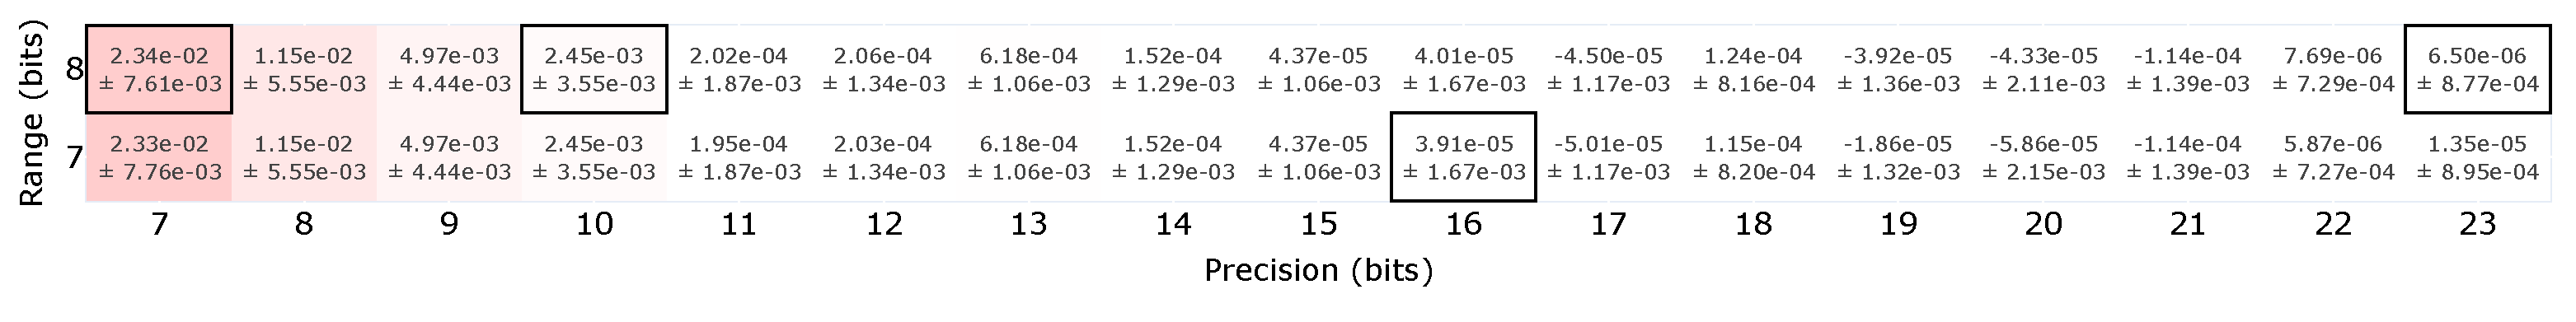
\includegraphics[width=\textwidth]{figures/0111-rigid-metric_rel_diff-mean.pdf}
	\end{subfigure}
	\begin{subfigure}[t]{\textwidth}
		\caption{[001x] Affine (MI)}
		\label{subfig:ants-search-001x}
		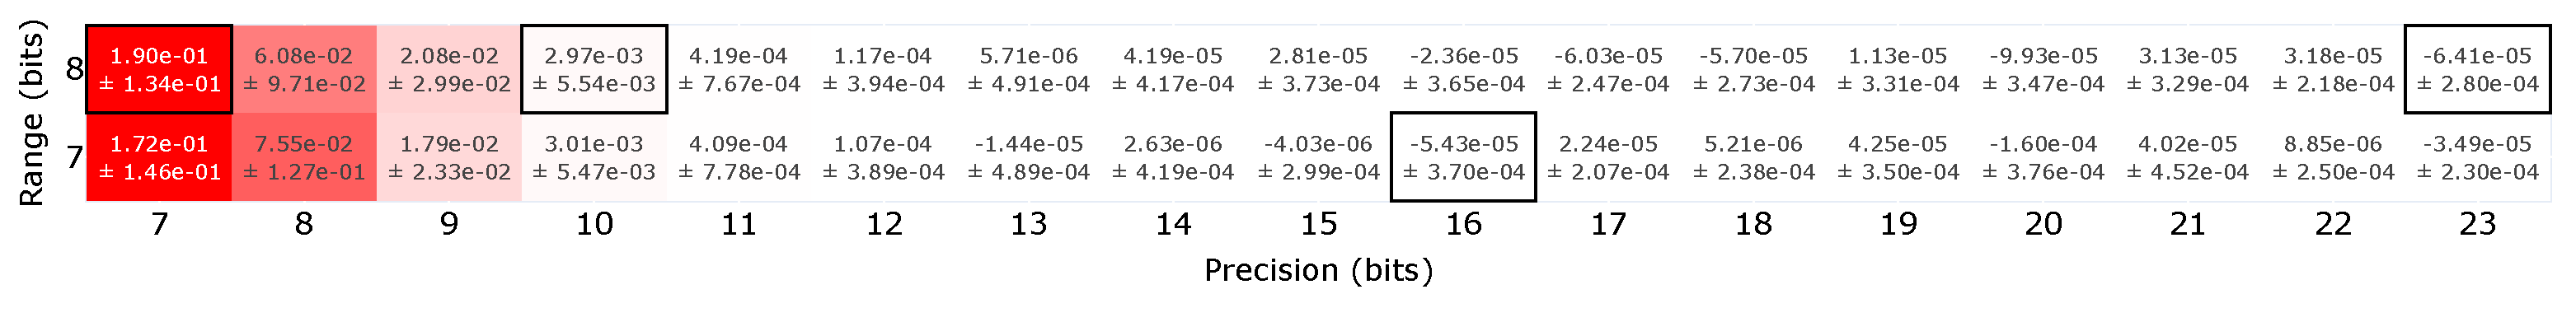
\includegraphics[width=\textwidth]{figures/0011-affine-metric_rel_diff-mean.pdf}
	\end{subfigure}
	\begin{subfigure}[t]{\textwidth}
		\caption{[0001] SyN (CC)}
		\label{subfig:ants-search-0001}
		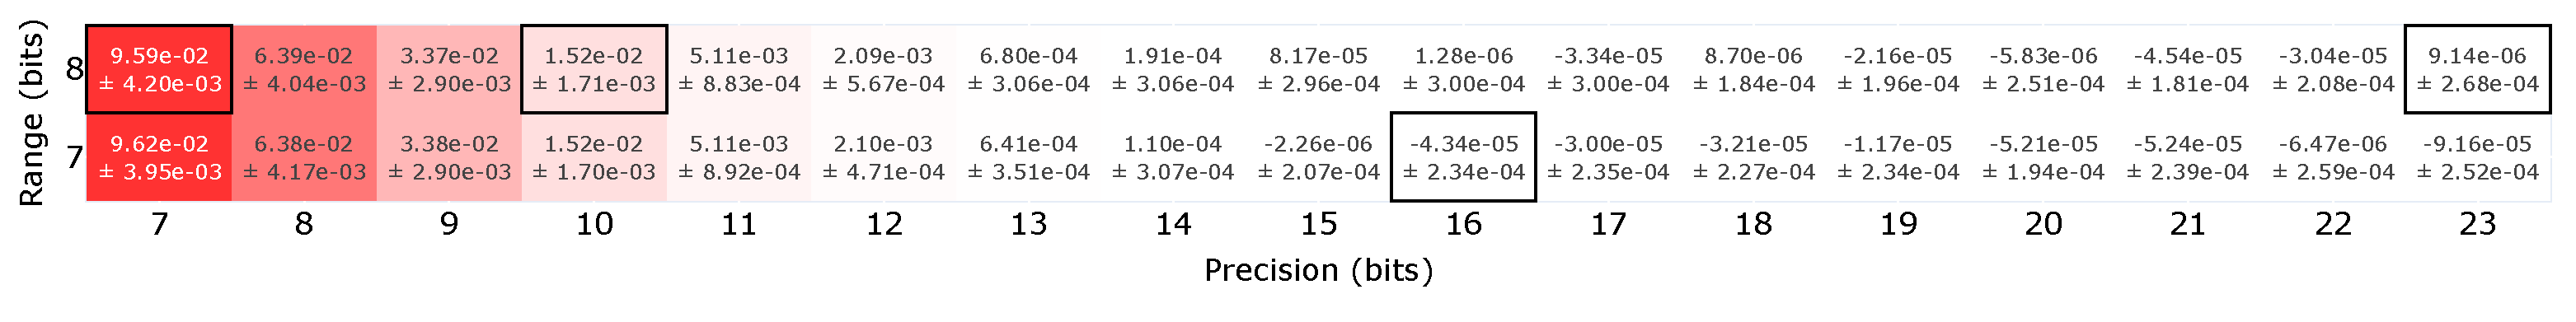
\includegraphics[width=\textwidth]{figures/0001-syn-metric_rel_diff-mean.pdf}
	\end{subfigure}
	\caption{No instrumentation in prior stages. The figure shows the relative difference in the similarity metric with respect to FP64---red is worse, green is better, and white denotes equivalence---with the color intensity representing the magnitude of the relative difference. We report the mean and standard deviation across subjects ($N=50$). We highlight data formats with hardware support: Float32~(r8-p23), Float24~(r7-p16), TensorFloat32~(r8-p10), and BFloat16~(r8-p7). The 4-bit binary encoding indicates whether we applied reduced precision at each stage: (1) initialization, (2) rigid, (3) affine, (4) SyN.}
	\label{fig:ants-space-search}
\end{figure*}

Overall our results indicate that using low-precision formats such as FP24 (r7-p16) and FP32 (r8-p23) has no significant impact on the accuracy of the registration---with a relative difference remaining below $10^{-5}$ for both formats. To remain within a relative difference threshold of $10^{-4}$ compared to FP64, the rigid and affine stages require at least 11 bits of precision, while the SyN stage requires at least 13 bits of precision---a much lower requirement than the default of 53-bit precision in FP64. 

Our results show no observable differences between exponent ranges of 7 and 8 bits. However, lowering the exponent range to 6 bits causes the application to crash or become unresponsive. Similarly, using 6-bit precision causes the pipeline to hang, regardless of the range. These behaviors appear across all stages and subjects.

We omit some configurations for the SyN and Affine stages, since the observed behaviors are consistent across all stages of a same type as long as the instrumentation of the stage remains the same.

% Our theoretical analysis in Section~\ref{sec:rp-theoretical-analysis} shows that the convergence of ANTs is mostly unaffected by FP32 and FP24 formats, while TF32 and BF16 formats have no convergence guarantee. Our empirical results (Figure~\ref{subfig:ants-0111}) align with this analysis; we observe no significant difference in the similarity metric when using FP32 and FP24 formats, while TF32 and BF16 formats show a significant degradation in the similarity metric.


\subsection{Current Stage Precision Dictates Accuracy}
Table ~\ref{tab:stage-accuracy} depicts the relative difference in accuracy of the SyN stage with and without instrumentation in BF16. The prior stages are all instrumented using BF16, leaving only the SyN stage to compare. Our results show a degradation in accuracy during the instrumented rigid and affine stage. This degradation is continued during the instrumented SyN stage, leading to a final relative difference of 8.68\% (average across subjects). However, for the non-instrumented version of the SyN stage, we observe accuracy recovery, even obtaining 0.54\% better similarity relative to FP64. This pattern is observed in other stages, independently of the prior stage instrumentation. Therefore, it suggests that only the instrumentation of the current stage is pertinent to the final similarity metric.


% Exception for the initialization step
\newcommand{\RedHL}[1]{\cellcolor[HTML]{FD6864}{\color[HTML]{333333} #1}}
\newcommand{\GreenHL}[1]{\cellcolor[HTML]{67FD9A}{\color[HTML]{333333} #1}}
\begin{table}[htb!]
\centering
\begin{tabular}{@{}llll@{}}
\toprule
\multicolumn{1}{c}{\textbf{Exp. ID}} & \multicolumn{1}{c}{\textbf{Rigid (MI)}} & \multicolumn{1}{c}{\textbf{Affine (MI)}} & \multicolumn{1}{c}{\textbf{SyN (CC)}} \\ \midrule
{\uline{011}\textbf{1}} & \RedHL{2.34e-02} & \RedHL{1.86e-01} & \RedHL{8.68e-02} \\
{\uline{011}\textbf{0}} & \RedHL{2.34e-02} & \RedHL{1.86e-01} & \GreenHL{-5.38e-03} \\ \bottomrule
\end{tabular}
\caption{Relative difference between \textbf{BF16} and FP64 for instrumented vs. non-instrument SyN stage. The prior rigid and affine stages are instrument with the same precision. We denote the Experiment ID as 0 (non-instrumented) and 1 (instrumented) for each stage. Green highlight indicates better performance with BF16 compared to FP64, while red is worse.}
\label{tab:stage-accuracy}
\end{table}

\subsection{$p_{min}$ Prediction and VPREC Estimation}
% TODO: This might be a bit repetitive with the method section on metric computation
Figure~\ref{fig:ants-pmin-ovserview} compares our $p_{min}$ prediction with the empirical results obtained using VPREC. For VPREC, we define $p_{min}$ by: (1) computing the relative metric difference of each data format with FP64, (2) compute the mean across subjects, (3) select the formats with average relative difference below the given threshold, and (4) select the minimum precision among those formats. By contstruction, the VPREC is monitonically increasing with iterations.

\begin{figure*}[htb!]
	\centering
	
\includegraphics[width=\textwidth]{figures/pmin-threshold-last-iteration/pmin-overview.pdf}
	\caption{$p_{min}$ prediction (dotted line) and VPREC estimation (solid colored lines). We report the average across subjects (N=50) per iteration. The different VPREC estimation represent the following relative difference thresholds: 1e-02 (1\%; blue), 5e-3 (0.5\%; orange), 1e-3 (0.1\%; green), and 1e-4 (0.01\%; magenta). For each threshold, we report its value (T), the area ratio percent where the our prediction is under (U) and over (O) the VPREC threshold curve. We highlight precision with hardware support as solid lightgreay horizontal lines.}
	\label{fig:ants-pmin-overview}
\end{figure*}

% TODO descrive the precision requirements from the esimated pmin.


In Figure~\ref{fig:ants-pmin-overview}, overall, our predicted $p_{min}$ (dash line) remain above the VPREC thresholds, except for the SyN levels 1 and 2. This indicates that the number of predicted bits is sufficient for convergence. 

Table~\ref{tab:area-ratio-summary} summarize the area ratio percent above and below the VPREC thresholds across all stages. For a relative difference of 1e-3 (0.1\%), our model underestimate the required number of bits by 11.57\% on average. However, we observed a large standard deviation across all values, indicating that our model accuracy varies significantly across stage-level combinations. Overall, our model overestimates significantly than it underestimates.

\begin{table}[htb!]
\centering
\begin{tabular}{@{}lll@{}}
\toprule
\multicolumn{1}{c}{\textbf{Threshold}} & \multicolumn{1}{c}{\textbf{Under}} & \multicolumn{1}{c}{\textbf{Over}} \\ \midrule
1e-2 & $6.15\pm6.90$ & $50.59\pm43.58$ \\
5e-3 & $7.41\pm7.03$ & $43.32\pm35.24$ \\
1e-3 & $11.57\pm9.75$ & $34.57\pm30.70$ \\
1e-4 & $16.79\pm11.40$ & $26.03\pm22.61$ \\ \bottomrule
\end{tabular}
\caption{Summary of the area ratio between our prediction curve and the different threshold curves, indicating when our prediction under (or over) estimated the number of precision required for convergence. We report the mean and standard deviation across all stage-level combinations.}
\label{tab:area-ratio-summary}
\end{table}

% remain below the precision provided by FP24 (16 bits), except for the first two rigid levels requiring up to 21 bits of precision. The rigid and affine stages exhibit similar $p_{min}$ requirements~($<$21), while the SyN stage is lower~($<$15).

% The required precision tends to increase with iterations, but remains similar across resolution levels within each stage. However, the precision in the earlier resolution levels (i.e., 1-2) tends to vary more. In contrast, the precision in the last two resolution levels (i.e., 3-4) is stable. Moreover, the last two levels tend to require lower precision than the first two levels.

% In early iterations ($<$10), our estimated $p_{min}$ values are consistently lower than those observed with VPREC. Our estimated $p_{min}$ values tends to be over the VPREC-observed values, providing a conservative estimate of the minimum precision required for convergence. For the SyN stage, our estimates align well with the VPREC results in level 1 and 4, but underestimate the precision required in levels 2 and 3.

% Our estimates show some steep spikes at certain iterations, particularly in the affine stage. In contrast, the VPREC results are stable across iterations.


% \subsection{Estimating theoretical bounds on ANTs convergence}
% Figure~\ref{fig:ants-pmin-min-max} shows the minimum data format precision required for ANTs to converge at each iteration. We compute $p_{min}$ using Equation~\ref{eq:hayford-pmin}. Our results indicate that the convergence of ANTs is mostly unaffected when using FP32 format, with only a minimal set of iterations lacking convergence guarantee. This suggests that FP32 could be used across the entire ANTs pipeline without loss in accuracy,resulting in significant speed up.

% The FP24 format exhibits lower convergence guarantee in the affine stage---level one, two, and three---especially for the last. The last rigid level show similar effect. By consequence, the format may be used to accelerate some registration stages---such as, rigid level 0, 1, and 2, and affine level 0---but may result in accuracy degradation when used across the entire pipeline.

% Using TF32 or BF16 provide no guarantee on the convergence of ANTs, across all stages and resolution levels. Thus, those data formats are not suitable to accelerate registration stages. However, future work could explore leveraging TF32 or BF16 to speed up a subset of early iterations within each stages, where the formats still guarantee convergence at those iterations.

% % TODO CLEANUP Only makes sense to keep if we want to discuss the boundaries in depth. However, the overview figure can include teh boundaries as well.

% % \begin{figure*}[htb!]
% % 	\centering
% % 	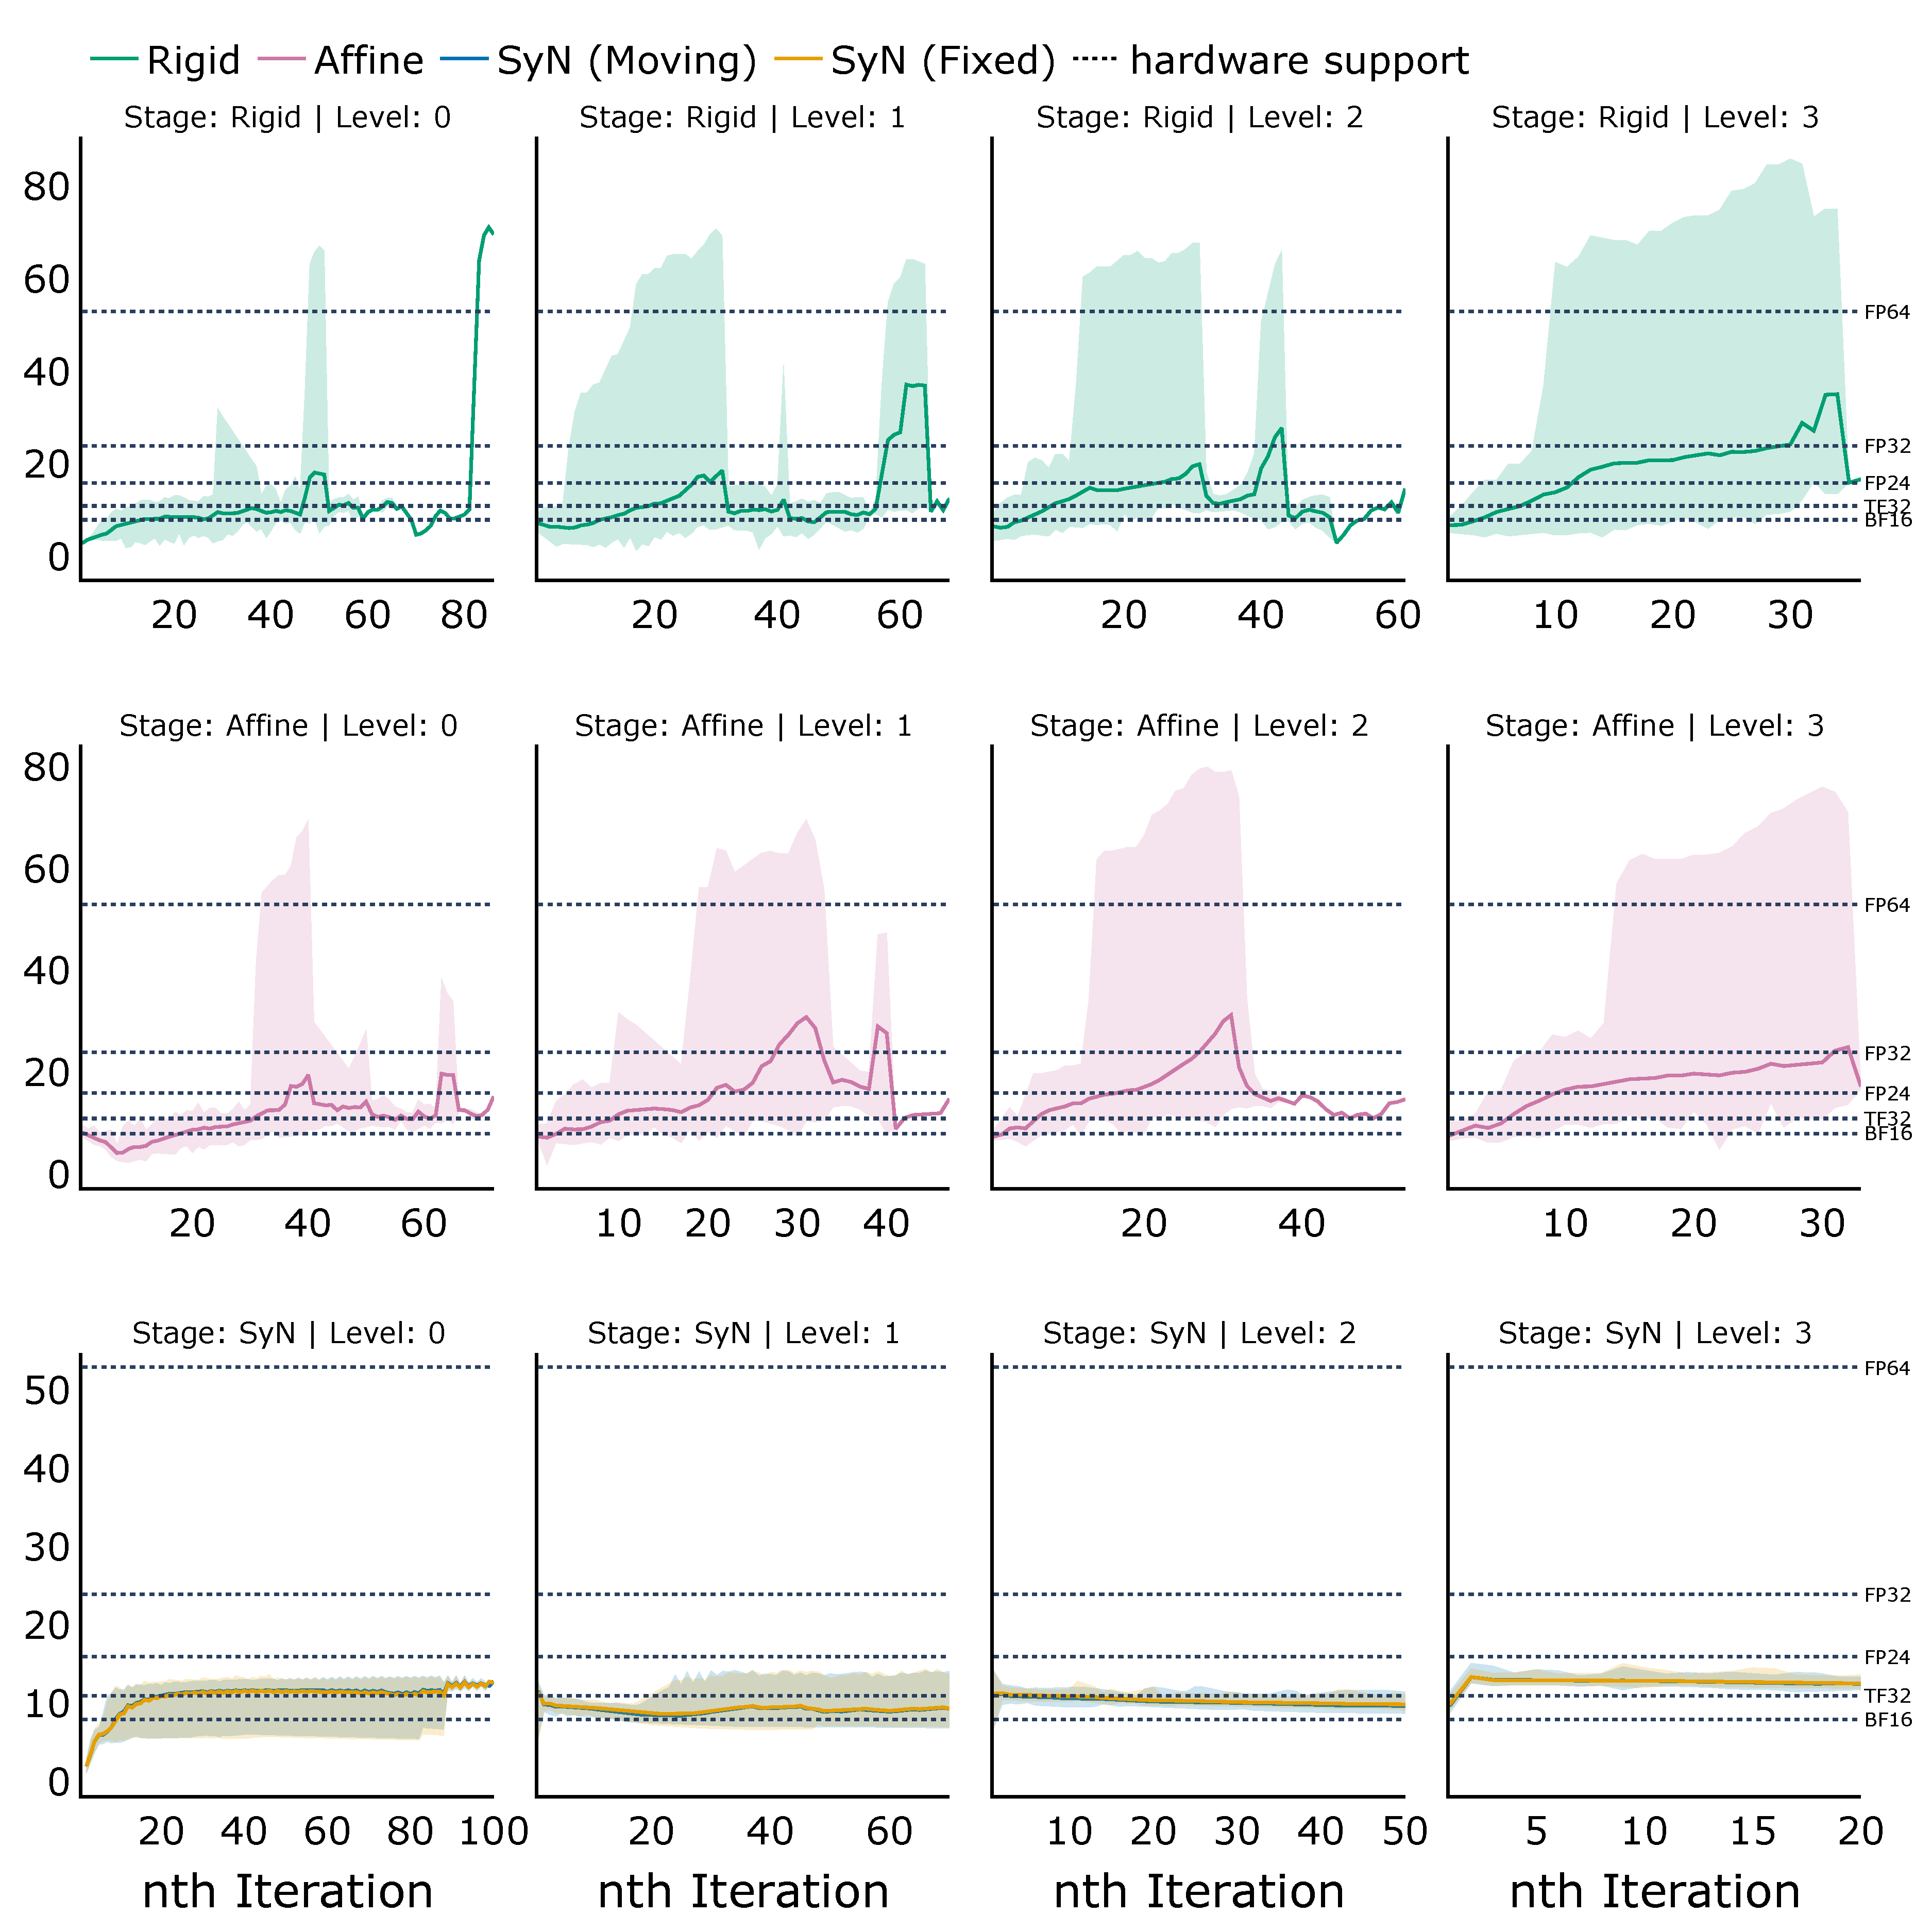
\includegraphics[width=\textwidth]{figures/pmin-min-max.pdf}
% % 	\caption{Estimated $p_{min}$ value computed as the average across subjects (N=50) per iteration. The min-max boundaries are depicted as shaded regions. We highlight precision with hardware support as dotted horizontal lines.}
% % 	\label{fig:ants-pmin-min-max}
% % \end{figure*}

% The current modification we made to ITK and the ANTs pipeline allow us to estimate a Lipschitz constant, loss gradient norm, and parameter norm at each iteration. While our modification works well for the rigid and affine stages, it fails to probe the SyN stage, which always returns a value of zero for the parameters norm. This is likely due to the different algorithm in SyN stage, which computes a displacement vector at each voxel rather than a transformation matrix. We plan to further investigate this issue and adapt our probing method to work with the SyN stage.

% Our current estimation of $p_{min}$ is based on a single subject. In future work, we plan to use an aggregation across all subjects to improve the estimation.


\section{Discussion}
\label{sec:discussion}
\subsection{Catastrophic Failure with Low Precision}
Preliminary results showed that using low precision (less than 14 bits) for the initial alignment often caused unrecoverable registration failures, resulting in large missing brain chunks. Consequently, we included only the \textit{1111} configuration—where all stages run in reduced precision—to evaluate this scenario explicitly.

We reduced the exponent and range down to 7 bits each (inclusively) as using 6 bits or less was resulting in the application crashing or hanging indefinitely. This is likely due to ITK not expected such low data format, which could result in the application following a different execution branch or failing to meeting a threshold during an iterative process.

\subsection{Theorem Assumptions}
The theorem from Hayford et al.~\cite{Hayford2024-kb} requires for the loss function to be convex. This is unlikely for complex real-world problem and is difficult to evaluate in practice. Our results showcase that although this assumption is likely unmet in ANTs registration, we can still leverage this simple model to accuratly predict the precision bits required for convergence. However, this is likely application specific, and further research could investigate the model on a collection of application to assess whether this assumption can be relaxed in practice.

\subsection{Performance Opportunity from $p_{min}$ Estimation}
Our current experiments incur large computational cost from simulating precison of each range-precision combination with VPREC. Leveraging our theoretical model to predict $p_{min}$ and subsequentially modify the precision during runtime would allow precision tuning without repeated execution, therefore enabling practical use of mixed precision in ANTs.

\subsection{Norm Choice}
We used the two-norm across all of our computations, consistant with the approach in~\cite{Hayford2024-kb}. While this ensure methodological alignment, we acknowledge that the norm two does not account for the different units and variability from our transformation parameters. Thus, we plan to investigate the impact from using a Mahalanobis norm that accounts for parameters scaling in future work.

\subsection{Mixed Precision Granularity}
Our results highlight significant potential benefits from using mixed precision at a stage-level granularity. However, even further performance gains could be obtained by leveraging mixed precision at a finer level---e.g., by varying precision per iteration (temporally) or code section (spatially). However, fine-grain mixed precision is challenging. First, casting overhead from frequent oscillation between data format would instead result in performance degradation. Second, implementing fine-grain tuning of precision remains technically challenging in large or complex codebase. 

A first avenue would be to implement our theoretical model in practice by inject the precision requirement at runtime. Additionally, our current experiments perform the similarity metric computation in double precision, to avoid runtime convergence issues. As implementing varying the ITK precision spatial would be technically chanlleging and may results in casting overhead, future work should investigate methods to compute the similarity metric at the same precision as other operation of during each iteration.

\subsection{Defining Accuracy Threshold}
While we compare our model against multiple accuracy thresholds, these remains fairly application specific. Future work could focus on a collection of analysis and study the impact of applying reduced precision to the clinical outcomes.

\subsection{Model Under and Over Prediction}
Our theoretical model is unlikely to predict the exact bit requirements at each iteration. On the one hand, over predictions preserve the convergence guarantee, but limit the potential speed up from lower bit formats. On the other hand, underprediction risk converge problem, by aggressively reducing the bit used.


\section{Conclusion}
\label{sec:conclusion}


\appendices

\section*{Appendix and the Use of Supplemental Files}
Appendices, if needed, appear before the acknowledgment. If an appendix is not
critical to the main message of the manuscript and is included only for thoroughness
or for reader reference, then consider submitting appendices as supplemental materials.
Supplementary files are available to readers through IEEE \emph{Xplore\textregistered}
at no additional cost to the authors but they do not appear in print versions.
Supplementary files must be uploaded in ScholarOne as supporting documents, but for
accepted papers they should be uploaded as Multimedia documents. Refer readers
to the supplementary files where appropriate within the manuscript text using footnotes.
\footnote{Supplementary materials are available in the supporting documents/multimedia tab.
Further instructions on footnote usage are in the Footnotes section on the next page.}

\section*{Acknowledgment}
The preferred spelling of the word ``acknowledgment'' in American English is 
without an ``e'' after the ``g.'' Use the singular heading even if you have 
many acknowledgments. Avoid expressions such as ``One of us (S.B.A.) would 
like to thank $\ldots$ .'' Instead, write ``F. A. Author thanks $\ldots$ .'' In most 
cases, sponsor and financial support acknowledgments are placed in the 
unnumbered footnote on the first page, not here.

\bibliography{paper.bib}
\bibliographystyle{IEEEtran}
\end{document}
